\tikzstyle{st}=[lightgray, fill, fill opacity=0.1] 
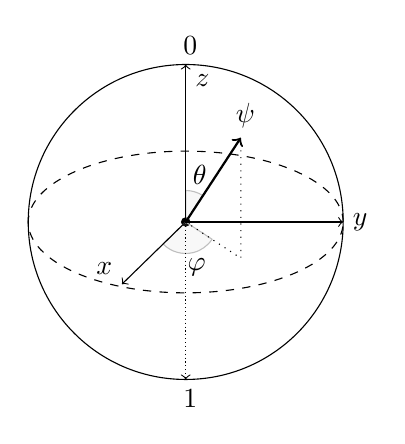
\begin{tikzpicture}
  \coordinate(o)at(0,0);
  \draw (o) circle (2cm);
  \draw [fill] (o) circle (1.5pt);%origin
  \draw [st] (o) -- (56.7:0.4) arc (56.7:90.:0.4) -- cycle;%theta angle
  \draw (0.18,0.6) node {$\theta$};
  \draw [st] (o) -- (-135.7:0.4) arc (-135.7:-33.2:0.4) -- cycle;%varphi angle
  \draw (0.14,-0.58) node {$\varphi$};
  \draw [->] (o) -- (-0.81,-0.79) node[above left]{\ $x$};%x
  \draw [->] (o) -- (2,0) node[right]{$y$};%y
  \draw [->] (o) -- (0,2) node[below right]{$z$} node[above]{\ $\ket{0}$};%z |0>
  \draw [rotate around={0.:(0.,0.)},dashed] (0,0) ellipse (2cm and 0.9cm);%ellipse
  \draw [thick,->](o) -- (0.70,1.07) node[above]{\ $\ket{\psi}$};%state vector
  \draw [densely dotted,->] (o) -- (0,-2) node[below]{\ $\ket{1}$};%-z |1>
  \draw [dotted] (o) -- (0.7,-0.46) -- (0.7,1);%triangle
\end{tikzpicture}
